\documentclass[legalpaper,11pt]{article}

\pagestyle{plain}

\usepackage[utf8]{inputenc}
\usepackage[T1]{fontenc}
\usepackage[spanish,es-tabla,es-nodecimaldot]{babel}
\usepackage[mathcal]{euscript}
\usepackage{amsmath,amsfonts,amssymb,latexsym,mathrsfs,
            multicol,anysize,graphicx,enumitem}
\usepackage{ragged2e}
\usepackage{float}
\usepackage{booktabs}
\usepackage[font=small,labelfont=bf]{caption}
\usepackage[round,authoryear]{natbib}
\usepackage{lmodern}
\usepackage[hidelinks]{hyperref}

%%%%%%%%%%%%%%%%%%%%%%%%%%%%%%%%%

\marginsize{2cm}{2cm}{2cm}{2cm}
\graphicspath{{figuras/}}
\setlength{\parskip}{0.35em}
\setlist{itemsep=0.15em, topsep=0.3em}

%%%%%%%%%%%%%%%%%%%%%%%%%%%%%%%%%%%%%%

\def\r{\mathbb{R}}
\def\n{\mathbb{N}}
\def\z{\mathbb{Z}}
\newcommand{\E}{\mathrm{E}}
\newcommand{\Var}{\mathrm{Var}}

% Generado automáticamente por R/02_exportar_latex.R. No editar a mano.
\newcommand{\gN}{2\,764}
\newcommand{\gFechaIni}{5 de enero de 2015}
\newcommand{\gFechaFin}{30 de diciembre de 2025}
\newcommand{\gOosIni}{3 de enero de 2024}
\newcommand{\gOosN}{500}
\newcommand{\gMedia}{0{,}044}
\newcommand{\gDE}{1{,}128}
\newcommand{\gMin}{-11{,}59}
\newcommand{\gMax}{9{,}99}
\newcommand{\gAsim}{-0{,}58}
\newcommand{\gCurt}{17{,}3}
\newcommand{\gJB}{23\,840}
\newcommand{\gLBr}{199{,}1}
\newcommand{\gLBrr}{2906}
\newcommand{\gARCHLM}{839{,}3}
\newcommand{\gMu}{0{,}0947}
\newcommand{\gOmega}{0{,}0222}
\newcommand{\gAlpha}{0{,}173}
\newcommand{\gBeta}{0{,}822}
\newcommand{\gNu}{5{,}54}
\newcommand{\gSEmu}{0{,}0104}
\newcommand{\gSEomega}{0{,}0060}
\newcommand{\gSEalpha}{0{,}024}
\newcommand{\gSEbeta}{0{,}021}
\newcommand{\gSEnu}{0{,}58}
\newcommand{\gNalpha}{0{,}177}
\newcommand{\gNbeta}{0{,}791}
\newcommand{\gLLt}{-3478{,}6}
\newcommand{\gLLn}{-3575{,}0}
\newcommand{\gDLL}{96{,}4}
\newcommand{\gPersist}{0{,}9945}
\newcommand{\gVidaMedia}{125}
\newcommand{\gVarInc}{4{,}03}
\newcommand{\gSigInc}{2{,}01}
\newcommand{\gVolInc}{31{,}9}
\newcommand{\gVolMuestral}{17{,}9}
\newcommand{\gEstricta}{-0{,}041}
\newcommand{\gCuarto}{1{,}165}
\newcommand{\gKappaZ}{6{,}89}
\newcommand{\gVTalpha}{0{,}158}
\newcommand{\gVTbeta}{0{,}823}
\newcommand{\gVTpersist}{0{,}981}
\newcommand{\gVTnu}{5{,}92}
\newcommand{\gVTll}{-3479{,}4}
\newcommand{\gSigmaUltimo}{0{,}61}
\newcommand{\gSigmaUno}{0{,}58}
\newcommand{\gSigmaUnoAnual}{9{,}2}
\newcommand{\gSigmaH}{1{,}76}
\newcommand{\gSigmaHvt}{1{,}12}
\newcommand{\gH}{250}
\newcommand{\gSEpers}{0{,}011}
\newcommand{\gICinf}{0{,}973}
\newcommand{\gICsup}{1{,}016}
\newcommand{\gZpers}{-0{,}49}
\newcommand{\gLBz}{6{,}82}
\newcommand{\gLBzp}{0{,}74}
\newcommand{\gLBzz}{12{,}54}
\newcommand{\gLBzzp}{0{,}13}
\newcommand{\gLMz}{13{,}98}
\newcommand{\gLMzp}{0{,}30}
\newcommand{\gSB}{19{,}66}
\newcommand{\gSBp}{$<0{,}001$}
\newcommand{\gSBt}{3{,}21}
\newcommand{\gSBtp}{0{,}001}
\newcommand{\gExcUno}{9}
\newcommand{\gEspUno}{5}
\newcommand{\gKupUno}{2{,}61}
\newcommand{\gKupUnop}{0{,}106}
\newcommand{\gChrUno}{2{,}94}
\newcommand{\gChrUnop}{0{,}230}
\newcommand{\gExcCinco}{36}
\newcommand{\gEspCinco}{25}
\newcommand{\gKupCinco}{4{,}51}
\newcommand{\gKupCincop}{0{,}034}
\newcommand{\gChrCinco}{4{,}68}
\newcommand{\gChrCincop}{0{,}096}
\newcommand{\gRugarch}{1.5.6}
\newcommand{\gRversion}{4.3.3}


%%%%%%%%%%%%%%%%%%%%%%%%%%%%%%%%%%%%%%

\begin{document}

\begin{minipage}{0.15\linewidth}

\includegraphics[width=25mm]{escudo.jpg}
\end{minipage}
\begin{minipage}{0.78\linewidth}
\large{\centerline{Universidad de Antioquia}}
\centerline{Facultad de Ciencias Exactas y Naturales}
\centerline{Instituto de Matemáticas}
\centerline{Seminario de Series de Tiempo I}
\end{minipage}

\vspace{0.9cm}
\begin{center}
{\Large\bfseries Modelos GARCH: volatilidad condicional, estacionariedad\\[2pt]
y aplicación al riesgo del índice S\&P 500}

\vspace{0.4cm}
Rafael Alexander Riatiga Durán \qquad Santiago Montoya Vanegas
\end{center}
\vspace{0.3cm}

%%%%%%%%%%%%%%%%%%%%%%%%%%%%%%%%%%%%%%
\noindent\textbf{Resumen.}
Los rendimientos financieros tienen media casi impredecible, pero su varianza cambia en el
tiempo y se agrupa en episodios de calma y de turbulencia. Este trabajo presenta el modelo
GARCH$(p,q)$ de \citet{bollerslev1986} como herramienta para describir y pronosticar esa
varianza condicional: su motivación a partir de los hechos estilizados, la interpretación de
sus parámetros y las condiciones de estacionariedad de segundo orden, estricta y de existencia
de momentos. Se aplica un GARCH(1,1) con innovaciones $t$ de Student a \gN{} rendimientos
diarios del ETF SPY (2015--2025). El modelo elimina la heterocedasticidad condicional de los
residuales y estima una persistencia $\hat\alpha_1+\hat\beta_1=\gPersist$, con vida media de
un choque de unos \gVidaMedia{} días; el proceso es estrictamente estacionario, la condición de
segundo orden se cumple en la estimación puntual aunque no puede rechazarse el caso integrado
$\alpha_1+\beta_1=1$, y su cuarto momento no es finito. Como uso práctico se pronostica la
volatilidad y se calcula el Valor en Riesgo (VaR) diario fuera de muestra: el VaR al 1\,\%
supera las pruebas de cobertura, mientras que al 5\,\% subestima el riesgo. Las limitaciones
encontradas (asimetría no capturada y nivel de largo plazo mal identificado cuando
$\alpha_1+\beta_1\approx 1$) señalan las extensiones naturales del modelo.

\medskip
\noindent\textbf{Palabras clave:} heterocedasticidad condicional, GARCH, volatilidad,
persistencia, estacionariedad, Valor en Riesgo, S\&P 500.

%%%%%%%%%%%%%%%%%%%%%%%%%%%%%%%%%%%%%%
\section{Introducción}

En un modelo clásico de series de tiempo, como un ARMA, el interés está en la media
condicional y se supone que el ruido tiene varianza constante. En las series financieras de
alta frecuencia ocurre casi lo contrario: los rendimientos están prácticamente incorrelacionados,
pero la magnitud de los movimientos de hoy anticipa la magnitud de los de mañana. Esa dependencia
no lineal es invisible para la función de autocorrelación de los rendimientos y es lo que
modelan los procesos ARCH \citep{engle1982} y su generalización GARCH \citep{bollerslev1986}.

La volatilidad es la variable central de la gestión de riesgo, de la valoración de opciones y
de la asignación de portafolios; por eso un modelo que la pronostique con pocos parámetros
tiene un uso inmediato. El trabajo sigue una ruta metodológica estándar: se verifica que los
datos presentan los hechos estilizados que motivan el modelo, se presenta su formulación y
sus propiedades, se estima y valida sobre los rendimientos diarios del S\&P 500, y se usa
para pronosticar la volatilidad y medir el riesgo mediante el VaR, evaluado fuera de muestra.
Los objetivos se precisan en la sección~\ref{sec:objetivos}.

%%%%%%%%%%%%%%%%%%%%%%%%%%%%%%%%%%%%%%
\section{Marco teórico}

\subsection{Motivación: hechos estilizados}
Las series de rendimientos $r_t=100\ln(P_t/P_{t-1})$ comparten regularidades empíricas
(\citealp{rossi2013}; \citealp[cap.~1]{francq2010}): (i) los precios no son estacionarios, pero los rendimientos sí
parecen serlo; (ii) los rendimientos tienen autocorrelación nula o muy débil; (iii) sus
cuadrados (o valores absolutos) están fuertemente autocorrelacionados, con decaimiento lento;
(iv) la volatilidad se agrupa: a grandes cambios les siguen grandes cambios; (v) la
distribución marginal es leptocúrtica, con colas más pesadas que la normal, y (vi) la
volatilidad tiende a aumentar más tras caídas que tras alzas de igual tamaño (efecto
apalancamiento). Los rasgos (ii)--(v) sugieren un proceso incorrelacionado pero
\emph{no independiente}, cuya varianza depende del pasado.

\subsection{Varianza condicional}
Sea $\mathcal{F}_{t-1}$ la información disponible hasta $t-1$. Se escribe
$r_t=\mu_t+\varepsilon_t$, con $\mu_t=\E(r_t\mid\mathcal{F}_{t-1})$ y
\begin{equation}\label{eq:eps}
\varepsilon_t=\sigma_t z_t,\qquad z_t\ \text{i.i.d.},\quad \E(z_t)=0,\quad \Var(z_t)=1,
\end{equation}
donde $\sigma_t>0$ es $\mathcal{F}_{t-1}$-medible. Entonces
$\E(\varepsilon_t\mid\mathcal{F}_{t-1})=0$ y
$\Var(\varepsilon_t\mid\mathcal{F}_{t-1})=\sigma_t^2$: la varianza \emph{condicional} cambia
con el tiempo aunque la incondicional pueda ser constante. Como $\{\varepsilon_t\}$ es una
diferencia de martingala, por la ley de esperanzas iteradas
$\mathrm{Cov}(\varepsilon_t,\varepsilon_{t+k})=0$ para $k\neq 0$; sin embargo,
$\varepsilon_t^2$ sí está autocorrelacionado. Esto reproduce los hechos (ii)--(iii).

\subsection{De ARCH a GARCH}
\citet{engle1982} propuso el ARCH$(q)$, $\sigma_t^2=\omega+\sum_{i=1}^{q}\alpha_i\varepsilon_{t-i}^2$,
en el que un choque grande eleva la varianza de los periodos siguientes. Reproducir la
persistencia observada exige un $q$ grande. \citet{bollerslev1986} añadió rezagos de la propia
varianza:
\begin{equation}\label{eq:garch}
\sigma_t^2=\omega+\sum_{i=1}^{q}\alpha_i\varepsilon_{t-i}^2+\sum_{j=1}^{p}\beta_j\sigma_{t-j}^2,
\qquad \omega>0,\ \alpha_i\ge 0,\ \beta_j\ge 0,
\end{equation}
restricciones suficientes para que $\sigma_t^2>0$. Dos representaciones ayudan a entenderlo.
Con $\nu_t=\varepsilon_t^2-\sigma_t^2$ (diferencia de martingala), $\varepsilon_t^2$ sigue un
ARMA$(\max(p,q),p)$:
\begin{equation}\label{eq:arma}
\varepsilon_t^2=\omega+\sum_{i=1}^{\max(p,q)}(\alpha_i+\beta_i)\,\varepsilon_{t-i}^2
+\nu_t-\sum_{j=1}^{p}\beta_j\nu_{t-j},
\end{equation}
lo que explica por qué la FAC de los cuadrados decae como la de un ARMA. Y, en el
GARCH(1,1), sustituyendo recursivamente,
\begin{equation}\label{eq:archinf}
\sigma_t^2=\frac{\omega}{1-\beta_1}+\alpha_1\sum_{k=1}^{\infty}\beta_1^{\,k-1}\varepsilon_{t-k}^2 ,
\end{equation}
es decir, un ARCH$(\infty)$ con pesos geométricos: tres parámetros resumen una memoria larga.

\subsection{Interpretación de los parámetros del GARCH(1,1)}
\begin{itemize}
  \item $\alpha_1$ (\emph{reacción}): cuánto se transmite la sorpresa de hoy,
  $\varepsilon_{t-1}^2$, a la varianza de mañana. Un $\alpha_1$ alto produce volatilidad
  ``nerviosa'', con picos marcados.
  \item $\beta_1$ (\emph{memoria}): qué fracción de la varianza de ayer se conserva.
  Un $\beta_1$ alto produce una volatilidad suave que decae lentamente.
  \item $\alpha_1+\beta_1$ (\emph{persistencia}): tasa a la que se disipa un choque sobre la
  varianza esperada; la \emph{vida media} de un choque es $\ln(0{,}5)/\ln(\alpha_1+\beta_1)$.
  \item $\omega$: junto con la persistencia fija el nivel de largo plazo,
  $\sigma^2=\E(\varepsilon_t^2)=\omega/(1-\alpha_1-\beta_1)$.
\end{itemize}

\subsection{Condiciones de estacionariedad}\label{sec:estac}
\textbf{Segundo orden.} Un proceso GARCH$(p,q)$ con coeficientes no negativos es
estacionario en covarianza si y solo si $\sum_i\alpha_i+\sum_j\beta_j<1$
\citep{bollerslev1986}; en ese caso $\Var(\varepsilon_t)=\omega/(1-\sum_i\alpha_i-\sum_j\beta_j)$.

\textbf{Estricta.} \citet{nelson1990} mostró que el GARCH(1,1) con $\omega>0$ tiene una única
solución estrictamente estacionaria y no anticipativa si y solo si
\begin{equation}\label{eq:estricta}
\gamma=\E\big[\ln(\beta_1+\alpha_1 z_t^2)\big]<0 .
\end{equation}
Por la desigualdad de Jensen, $\gamma\le\ln\E(\beta_1+\alpha_1z_t^2)=\ln(\alpha_1+\beta_1)$, de
modo que la condición de segundo orden implica la estricta, pero no al revés. En particular el
IGARCH(1,1), con $\alpha_1+\beta_1=1$, es estrictamente estacionario con varianza infinita. Para
el caso general $(p,q)$ la condición es que el mayor exponente de Lyapunov de la representación
vectorial del modelo sea negativo \citep{bougerol1992,francq2010}.

\textbf{Momentos de orden cuatro.} Si $\kappa_z=\E(z_t^4)$, el GARCH(1,1) tiene cuarto momento
finito si y solo si $(\alpha_1+\beta_1)^2+(\kappa_z-1)\alpha_1^2<1$, y entonces
\begin{equation}\label{eq:curtosis}
\kappa_\varepsilon=\frac{\E(\varepsilon_t^4)}{[\E(\varepsilon_t^2)]^2}
=\kappa_z\,\frac{1-(\alpha_1+\beta_1)^2}{1-(\alpha_1+\beta_1)^2-(\kappa_z-1)\alpha_1^2}>\kappa_z ,
\end{equation}
así que el modelo genera colas más pesadas que las de $z_t$ aun cuando $z_t$ es normal
($\kappa_z=3$): la heterocedasticidad condicional explica parte de la leptocurtosis.

\subsection{Pronóstico}
Bajo estacionariedad de segundo orden, el pronóstico a $k$ pasos de un GARCH(1,1) es
\begin{equation}\label{eq:pronostico}
\E_t\big(\sigma_{t+k}^2\big)=\sigma^2+(\alpha_1+\beta_1)^{k-1}\big(\sigma_{t+1}^2-\sigma^2\big),
\end{equation}
que converge geométricamente al nivel de largo plazo $\sigma^2$ a la tasa $\alpha_1+\beta_1$.

\subsection{Estimación}
Los parámetros se estiman por máxima verosimilitud condicional. Con la cuasi-verosimilitud
gaussiana, $\ell_n(\theta)=-\tfrac12\sum_t\big[\ln\sigma_t^2(\theta)+\varepsilon_t^2/\sigma_t^2(\theta)\big]$,
el estimador es consistente y asintóticamente normal aunque $z_t$ no sea normal, bajo
estacionariedad estricta y $\E(z_t^4)<\infty$ para la normalidad \citep{francq2004}; la
inferencia usa errores estándar robustos tipo sándwich \citep{bollerslev1992}. Si se supone
$z_t\sim t_\nu$ estandarizada se gana eficiencia, a cambio de depender de que la densidad sea
correcta \citep[cap.~9]{francq2010}.

\subsection{Uso en riesgo: Valor en Riesgo}
El VaR al nivel $a$ es el cuantil $a$ de la distribución condicional del rendimiento:
$\mathrm{VaR}_{t+1}(a)=\mu+\sigma_{t+1}\,q_a$, con
$q_a=t_\nu^{-1}(a)\sqrt{(\nu-2)/\nu}$ para innovaciones $t$ estandarizadas. Un VaR bien
calibrado debe ser excedido en una fracción $a$ de los días (cobertura incondicional,
prueba de \citealp{kupiec1995}) y las excedencias no deben agruparse (cobertura condicional,
prueba de \citealp{christoffersen1998}).

%%%%%%%%%%%%%%%%%%%%%%%%%%%%%%%%%%%%%%
\section{Objetivos}\label{sec:objetivos}

\textbf{General.} Estudiar el modelo GARCH como modelo de la varianza condicional de series
financieras y aplicarlo al pronóstico de la volatilidad y la medición del riesgo del índice
S\&P 500.

\textbf{Específicos.}
\begin{enumerate}[label=\arabic*.]
  \item Verificar en los rendimientos del S\&P 500 los hechos estilizados que motivan el modelo.
  \item Presentar la formulación del GARCH$(p,q)$, la interpretación de sus parámetros y sus
  condiciones de estacionariedad.
  \item Seleccionar, estimar y validar un modelo GARCH para los rendimientos diarios, y
  contrastar las condiciones teóricas con los parámetros estimados.
  \item Pronosticar la volatilidad y evaluar fuera de muestra el VaR derivado del modelo.
\end{enumerate}

%%%%%%%%%%%%%%%%%%%%%%%%%%%%%%%%%%%%%%
\section{Metodología}

\textbf{Datos.} Precios de cierre diarios del ETF SPY, réplica del S\&P 500, entre el
\gFechaIni{} y el \gFechaFin{} \citep{twelvedata}, con los que se calculan \gN{} rendimientos
logarítmicos porcentuales. Se usa el ETF porque es un activo negociable con la misma dinámica
del índice; los precios no se ajustan por dividendos, cuyo efecto (cerca de 0,3\,\% por
trimestre) es pequeño frente a la volatilidad diaria.

\textbf{Procedimiento.}
\begin{enumerate}[label=\arabic*.]
  \item \emph{Identificación}: estadísticos descriptivos, prueba de normalidad de
  \citet{jarque1980}, FAC de $r_t$ y $r_t^2$, pruebas de \citet{ljung1978} y ARCH-LM de
  \citet{engle1982}.
  \item \emph{Selección}: media constante y modelos GARCH$(p,q)$ con $p,q\le 2$, con
  innovaciones normales y $t$ de Student, comparados por AIC y BIC.
  \item \emph{Estimación}: máxima verosimilitud con errores estándar robustos;
  cálculo de la persistencia, la vida media, el nivel de largo plazo y las condiciones de
  estacionariedad. La condición~\eqref{eq:estricta} se evalúa por Monte Carlo con $10^6$
  extracciones de la $t$ estimada. Como análisis de sensibilidad se reestima con
  \emph{variance targeting} \citep{engle1996}, que fija $\sigma^2$ en la varianza muestral.
  \item \emph{Diagnóstico} sobre los residuales estandarizados $\hat z_t=\hat\varepsilon_t/\hat\sigma_t$:
  Ljung-Box sobre $\hat z_t$ y $\hat z_t^2$, ARCH-LM y prueba de sesgo de signo de
  \citet{engle1993}.
  \item \emph{Pronóstico y uso}: pronóstico de $\sigma_{t+k}$ para $k=1,\dots,\gH$ con
  \eqref{eq:pronostico}; VaR a un paso al 1\,\% y 5\,\% sobre los últimos \gOosN{} días
  (desde el \gOosIni), con ventana móvil y reestimación cada 25 días, evaluado con las
  pruebas de Kupiec y Christoffersen.
\end{enumerate}

\textbf{Herramientas.} R \gRversion{} \citep{rcore}, con el paquete \texttt{rugarch}
\gRugarch{} \citep{ghalanos} para la estimación, el pronóstico y el \emph{backtesting}, y
\texttt{tseries} y \texttt{FinTS} para las pruebas. El código acompaña este documento y es
reproducible.

%%%%%%%%%%%%%%%%%%%%%%%%%%%%%%%%%%%%%%
\section{Aplicación}

\subsection{Los datos presentan los hechos estilizados}
La figura~\ref{fig:datos} muestra un precio con tendencia y unos rendimientos que oscilan
alrededor de cero con episodios de turbulencia muy marcados: el choque de la pandemia en marzo
de 2020, la corrección de 2022 y la caída por los anuncios arancelarios de abril de 2025.
La tabla~\ref{tab:desc} confirma la leptocurtosis (curtosis de \gCurt, frente a 3 de la
normal) y una asimetría negativa leve; la normalidad se rechaza con holgura.

\begin{figure}[H]
\centering
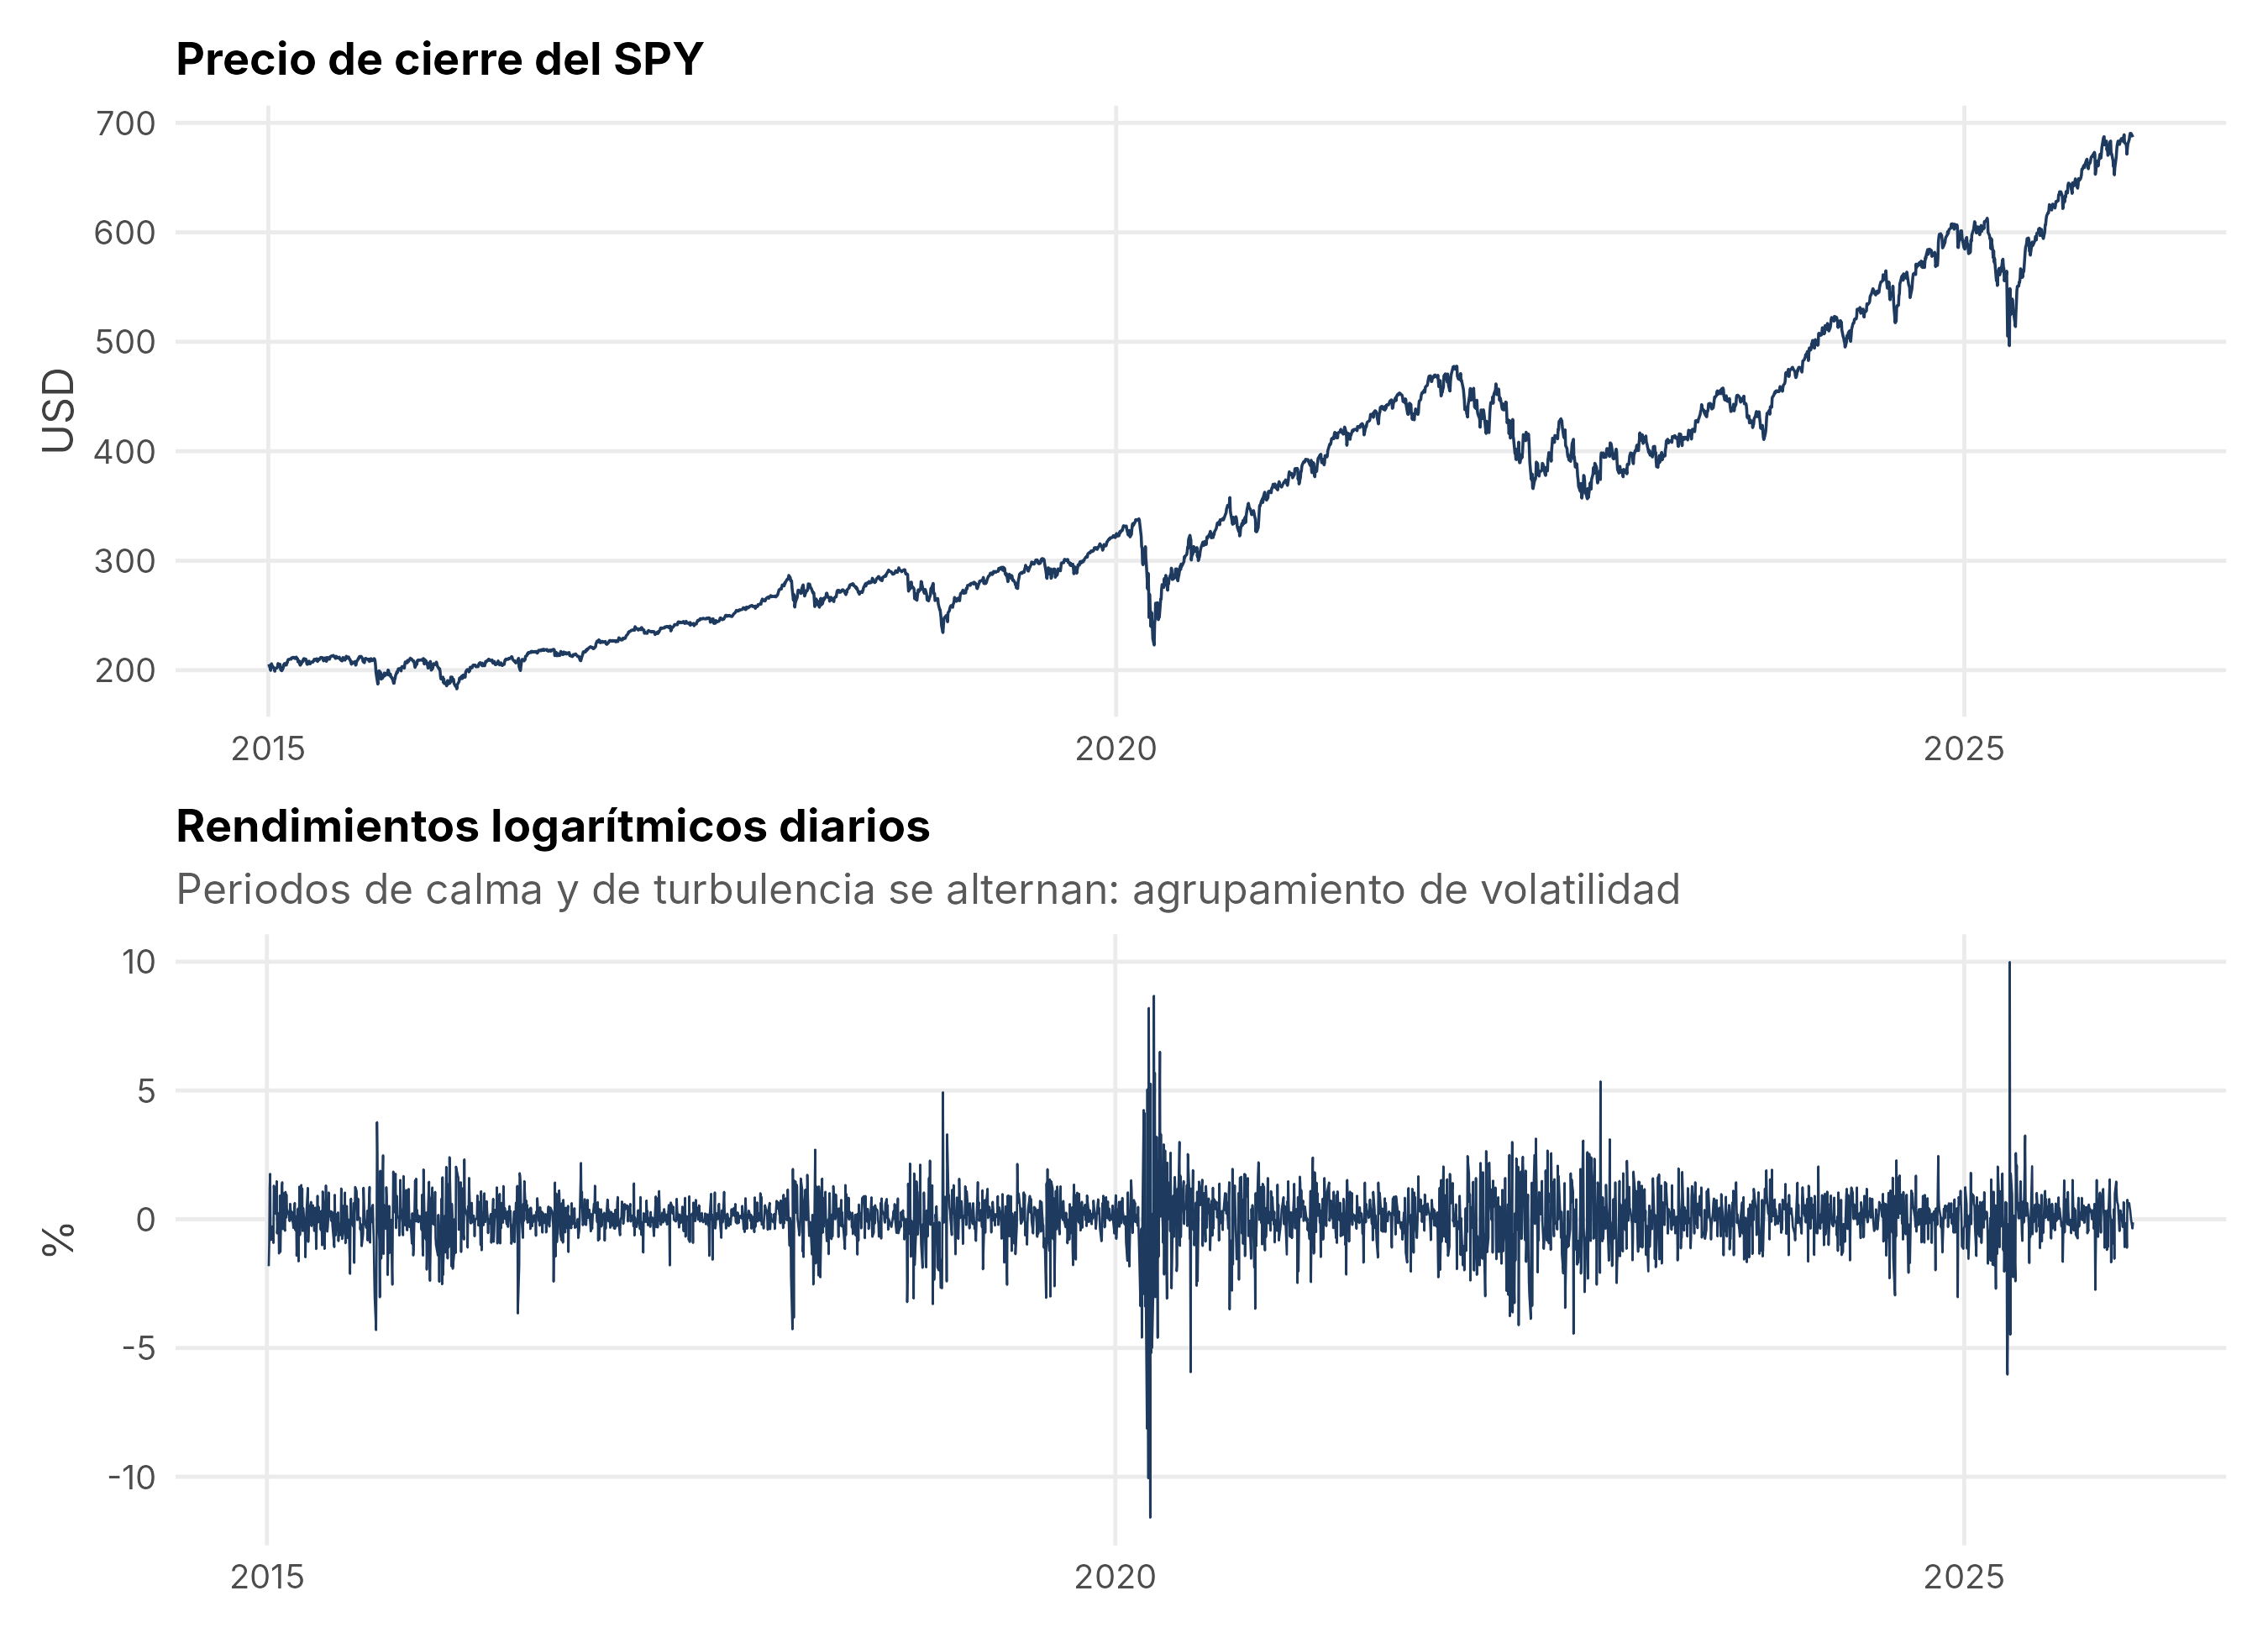
\includegraphics[width=0.88\linewidth]{f1_precio_rendimientos.png}
\caption{Precio de cierre y rendimientos logarítmicos diarios del SPY, 2015--2025.}
\label{fig:datos}
\end{figure}

\begin{table}[H]
\centering\small
\caption{Estadísticos descriptivos de $r_t$ (\%) y pruebas de identificación.}
\label{tab:desc}
\begin{tabular}{lr@{\hspace{2.2em}}lrr}
\toprule
Estadístico & Valor & Prueba & Estadístico & $p$-valor \\
\midrule
Media (\%) & 0{,}044 & Jarque-Bera & 23840{,}1 & $<0{,}001$ \\
Desv. estándar (\%) & 1{,}128 & Ljung-Box $Q(10)$, $r_t$ & 199{,}1 & $<0{,}001$ \\
Mínimo (\%) & -11{,}59 & Ljung-Box $Q(10)$, $r_t^2$ & 2906{,}2 & $<0{,}001$ \\
Máximo (\%) & 9{,}99 & ARCH-LM(12) & 839{,}3 & $<0{,}001$ \\
Asimetría & -0{,}58 & & & \\
Curtosis & 17{,}33 & & & \\
\bottomrule
\end{tabular}

\end{table}

La figura~\ref{fig:fac} es el argumento central a favor del modelo: la FAC de $r_t$ tiene
valores pequeños (los mayores, de signo alterno, provienen de 2020), mientras que la de
$r_t^2$ es grande, positiva y decae lentamente, como predice la representación
ARMA~\eqref{eq:arma}. Las pruebas de Ljung-Box sobre $r_t^2$ ($Q=\gLBrr$) y ARCH-LM
($\gARCHLM$) rechazan la homocedasticidad condicional. El rechazo de Ljung-Box sobre $r_t$
debe leerse con cautela: bajo heterocedasticidad condicional las bandas usuales
$\pm1{,}96/\sqrt n$ subestiman la varianza de las autocorrelaciones muestrales
\citep[cap.~5]{francq2010}; por eso se adopta una media constante y se verifica su
suficiencia sobre los residuales estandarizados.

\begin{figure}[H]
\centering
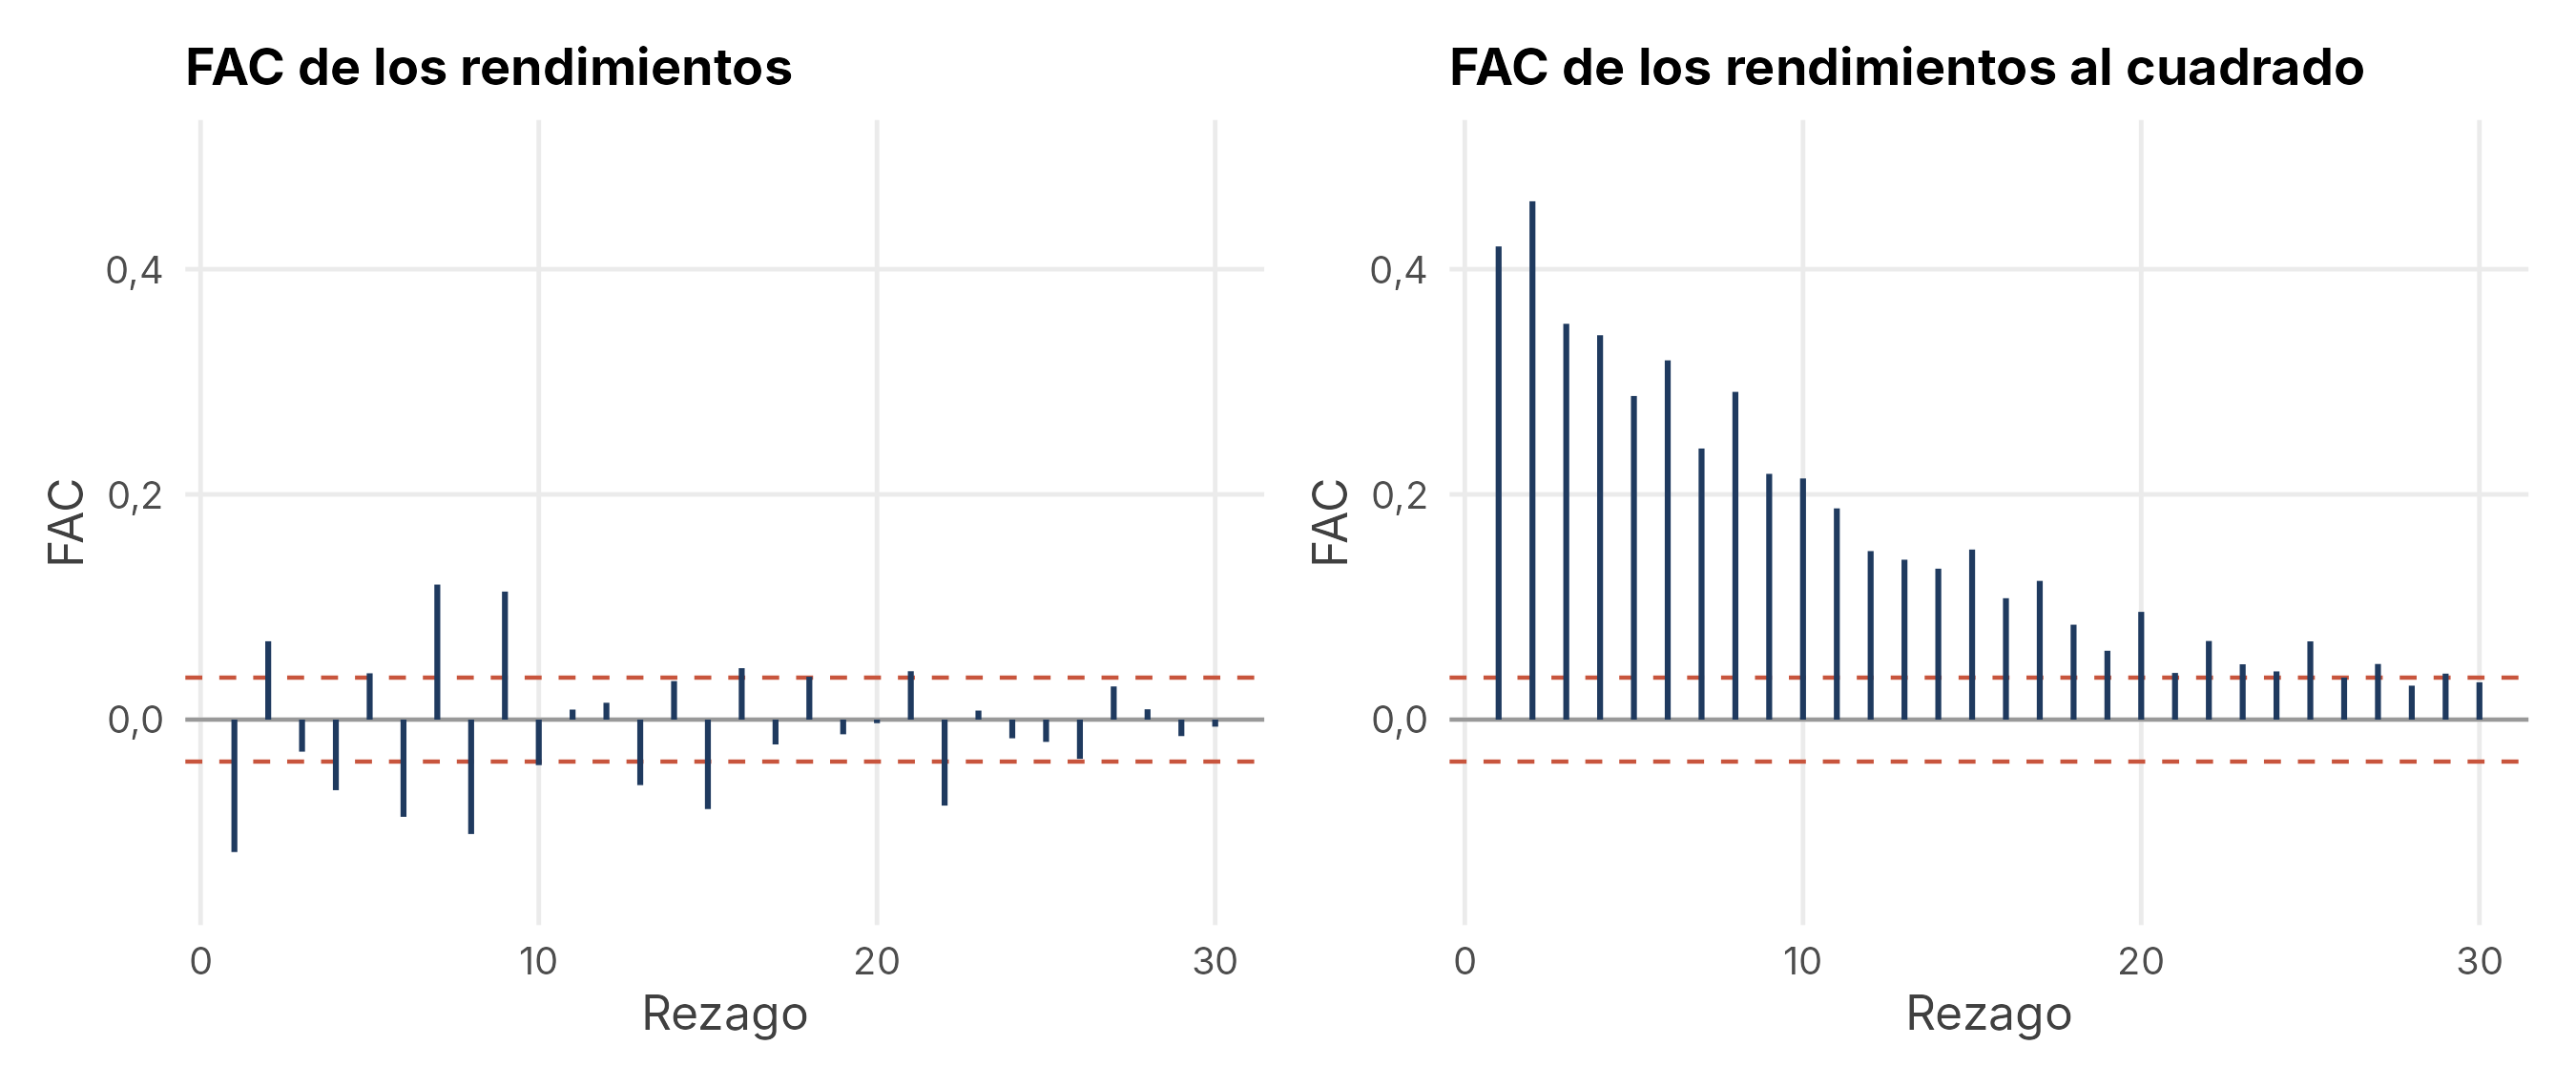
\includegraphics[width=0.88\linewidth]{f2_fac_r_r2.png}
\caption{FAC muestral de los rendimientos y de sus cuadrados, con bandas $\pm1{,}96/\sqrt{n}$.}
\label{fig:fac}
\end{figure}

\subsection{Selección y estimación}
En la tabla~\ref{tab:sel}, con cualquiera de las dos distribuciones, aumentar los órdenes
apenas cambia la verosimilitud y ambos criterios penalizan esos parámetros: el GARCH(1,1) es
suficiente, como es habitual en series de índices. La distribución $t$ mejora la
log-verosimilitud en \gDLL{} puntos con un solo parámetro adicional. Se elige el GARCH(1,1)
con innovaciones $t$.

\begin{table}[H]
\centering\small
\caption{Criterios de información (por observación) de los modelos candidatos.}
\label{tab:sel}
\begin{tabular}{llrrr}
\toprule
Modelo & Distribución & $\ln L$ & AIC & BIC \\
\midrule
GARCH(1,1) & Normal & -3574{,}98 & 2{,}5897 & 2{,}5983 \\
GARCH(1,2) & Normal & -3574{,}90 & 2{,}5904 & 2{,}6011 \\
GARCH(2,1) & Normal & -3574{,}90 & 2{,}5904 & 2{,}6011 \\
GARCH(2,2) & Normal & -3574{,}90 & 2{,}5911 & 2{,}6040 \\
\midrule
GARCH(1,1) & t-Student & -3478{,}62 & 2{,}5207 & \textbf{2{,}5314} \\
GARCH(1,2) & t-Student & -3478{,}54 & 2{,}5214 & 2{,}5342 \\
GARCH(2,1) & t-Student & -3478{,}79 & 2{,}5216 & 2{,}5344 \\
GARCH(2,2) & t-Student & -3478{,}49 & 2{,}5221 & 2{,}5371 \\
\bottomrule
\end{tabular}

\end{table}

\begin{table}[H]
\centering\small
\caption{Estimación del GARCH(1,1) con media constante. Errores estándar robustos entre paréntesis.}
\label{tab:est}
\begin{tabular}{lr@{\,}lr@{\,}l}
\toprule
 & \multicolumn{2}{c}{$t$-Student} & \multicolumn{2}{c}{Normal} \\
\cmidrule(lr){2-3}\cmidrule(lr){4-5}
Parámetro & Estimación & (EE) & Estimación & (EE) \\
\midrule
$\mu$ & 0{,}0947 & (0{,}0104) & 0{,}0798 & (0{,}0129) \\
$\omega$ & 0{,}0222 & (0{,}0060) & 0{,}0395 & (0{,}0098) \\
$\alpha_1$ & 0{,}173 & (0{,}024) & 0{,}177 & (0{,}028) \\
$\beta_1$ & 0{,}822 & (0{,}021) & 0{,}791 & (0{,}027) \\
$\nu$ & 5{,}54 & (0{,}58) & -- &  \\
\midrule
$\alpha_1+\beta_1$ & 0{,}9945 & & 0{,}9689 & \\
$\ln L$ & -3478{,}62 & & -3574{,}98 & \\
\bottomrule
\end{tabular}

\end{table}

\textbf{Interpretación.} Todos los parámetros son significativos (tabla~\ref{tab:est}).
Con $\hat\alpha_1=\gAlpha$, un rendimiento inesperado de 2\,\% (al cuadrado, 4) eleva la
varianza del día siguiente en cerca de $0{,}69$ puntos porcentuales al cuadrado; con
$\hat\beta_1=\gBeta$, el 82\,\% de la varianza de ayer se conserva. La persistencia
$\hat\alpha_1+\hat\beta_1=\gPersist$ implica una vida media de unos \gVidaMedia{} días hábiles:
los choques de volatilidad tardan meses en disiparse. $\hat\nu=\gNu$ indica colas pesadas en las
innovaciones mismas, no solo en la distribución marginal. Las estimaciones de $\alpha_1$ y
$\beta_1$ bajo la normal (cuasi-verosimilitud gaussiana) son cercanas, lo que respalda que la
dinámica estimada no depende de la elección de la densidad.

\subsection{Contraste con las condiciones teóricas}
La tabla~\ref{tab:estac} evalúa las condiciones de la sección~\ref{sec:estac} con los valores estimados.
Con los valores puntuales, el proceso es estacionario de segundo orden y en sentido estricto
($\hat\gamma=\gEstricta<0$). Sin embargo, el error estándar robusto de
$\hat\alpha_1+\hat\beta_1$ es \gSEpers{} y su intervalo de confianza del 95\,\%,
$(\gICinf;\ \gICsup)$, contiene a 1 ($z=\gZpers$ para $H_0:\alpha_1+\beta_1=1$): los datos no
permiten afirmar con seguridad estadística la estacionariedad de segundo orden. La estricta, en
cambio, se mantiene incluso en el caso integrado (sección~\ref{sec:estac}). Por otra parte, con $\kappa_z=3(\nu-2)/(\nu-4)=\gKappaZ$, la condición
de cuarto momento vale \gCuarto{} $>1$: la curtosis~\eqref{eq:curtosis} no es finita, coherente
con la curtosis muestral muy alta.

\begin{table}[H]
\centering\small
\caption{Condiciones de estacionariedad y momentos evaluadas en las estimaciones.}
\label{tab:estac}
\begin{tabular}{lrc}
\toprule
Condición & Valor & ¿Se cumple? \\
\midrule
Segundo orden: $\alpha_1+\beta_1<1$ & 0{,}9945 & Sí \\
Estricta: $\mathrm{E}\ln(\beta_1+\alpha_1 z_t^2)<0$ & -0{,}041 & Sí \\
Cuarto momento: $(\alpha_1+\beta_1)^2+(\kappa_z-1)\alpha_1^2<1$ & 1{,}165 & No \\
\midrule
Vida media de un choque (días) & 125 & \\
Volatilidad anual de largo plazo implícita (\%) & 31{,}9 & \\
Volatilidad anual muestral (\%) & 17{,}9 & \\
\bottomrule
\end{tabular}

\end{table}

La última fila revela una tensión importante. Con $\hat\alpha_1+\hat\beta_1$ tan cercano a 1, el
cociente $\hat\omega/(1-\hat\alpha_1-\hat\beta_1)$ amplifica cualquier error de estimación: el
nivel de largo plazo implícito (\gVolInc\,\% anual) casi duplica la volatilidad muestral
(\gVolMuestral\,\%). Al imponer \emph{variance targeting} se obtiene $\hat\alpha_1=\gVTalpha$,
$\hat\beta_1=\gVTbeta$ y persistencia \gVTpersist, con una log-verosimilitud
(\gVTll) casi igual a la del modelo libre (\gLLt): los datos apenas distinguen ambos niveles
de largo plazo. Una persistencia tan alta también puede reflejar cambios estructurales no
modelados en la varianza \citep{lamoureux1990}.

\subsection{Diagnóstico}
La volatilidad condicional estimada (figura~\ref{fig:vol}) sigue de cerca los episodios de
turbulencia y retorna lentamente a niveles bajos. Según la tabla~\ref{tab:diag}, no queda
autocorrelación en $\hat z_t$ ni en $\hat z_t^2$, ni efecto ARCH remanente: el modelo captura la
dinámica de la varianza y la media constante es adecuada. El gráfico QQ (figura~\ref{fig:diag})
muestra que la $t$ ajusta bien el centro y la cola izquierda moderada, con desviaciones en los
extremos. La prueba de sesgo de signo, en cambio, rechaza ($p$ \gSBp): el signo del choque
influye en la volatilidad futura, algo que el GARCH, al depender solo de $\varepsilon_{t-1}^2$,
no puede capturar.

\begin{figure}[H]
\centering
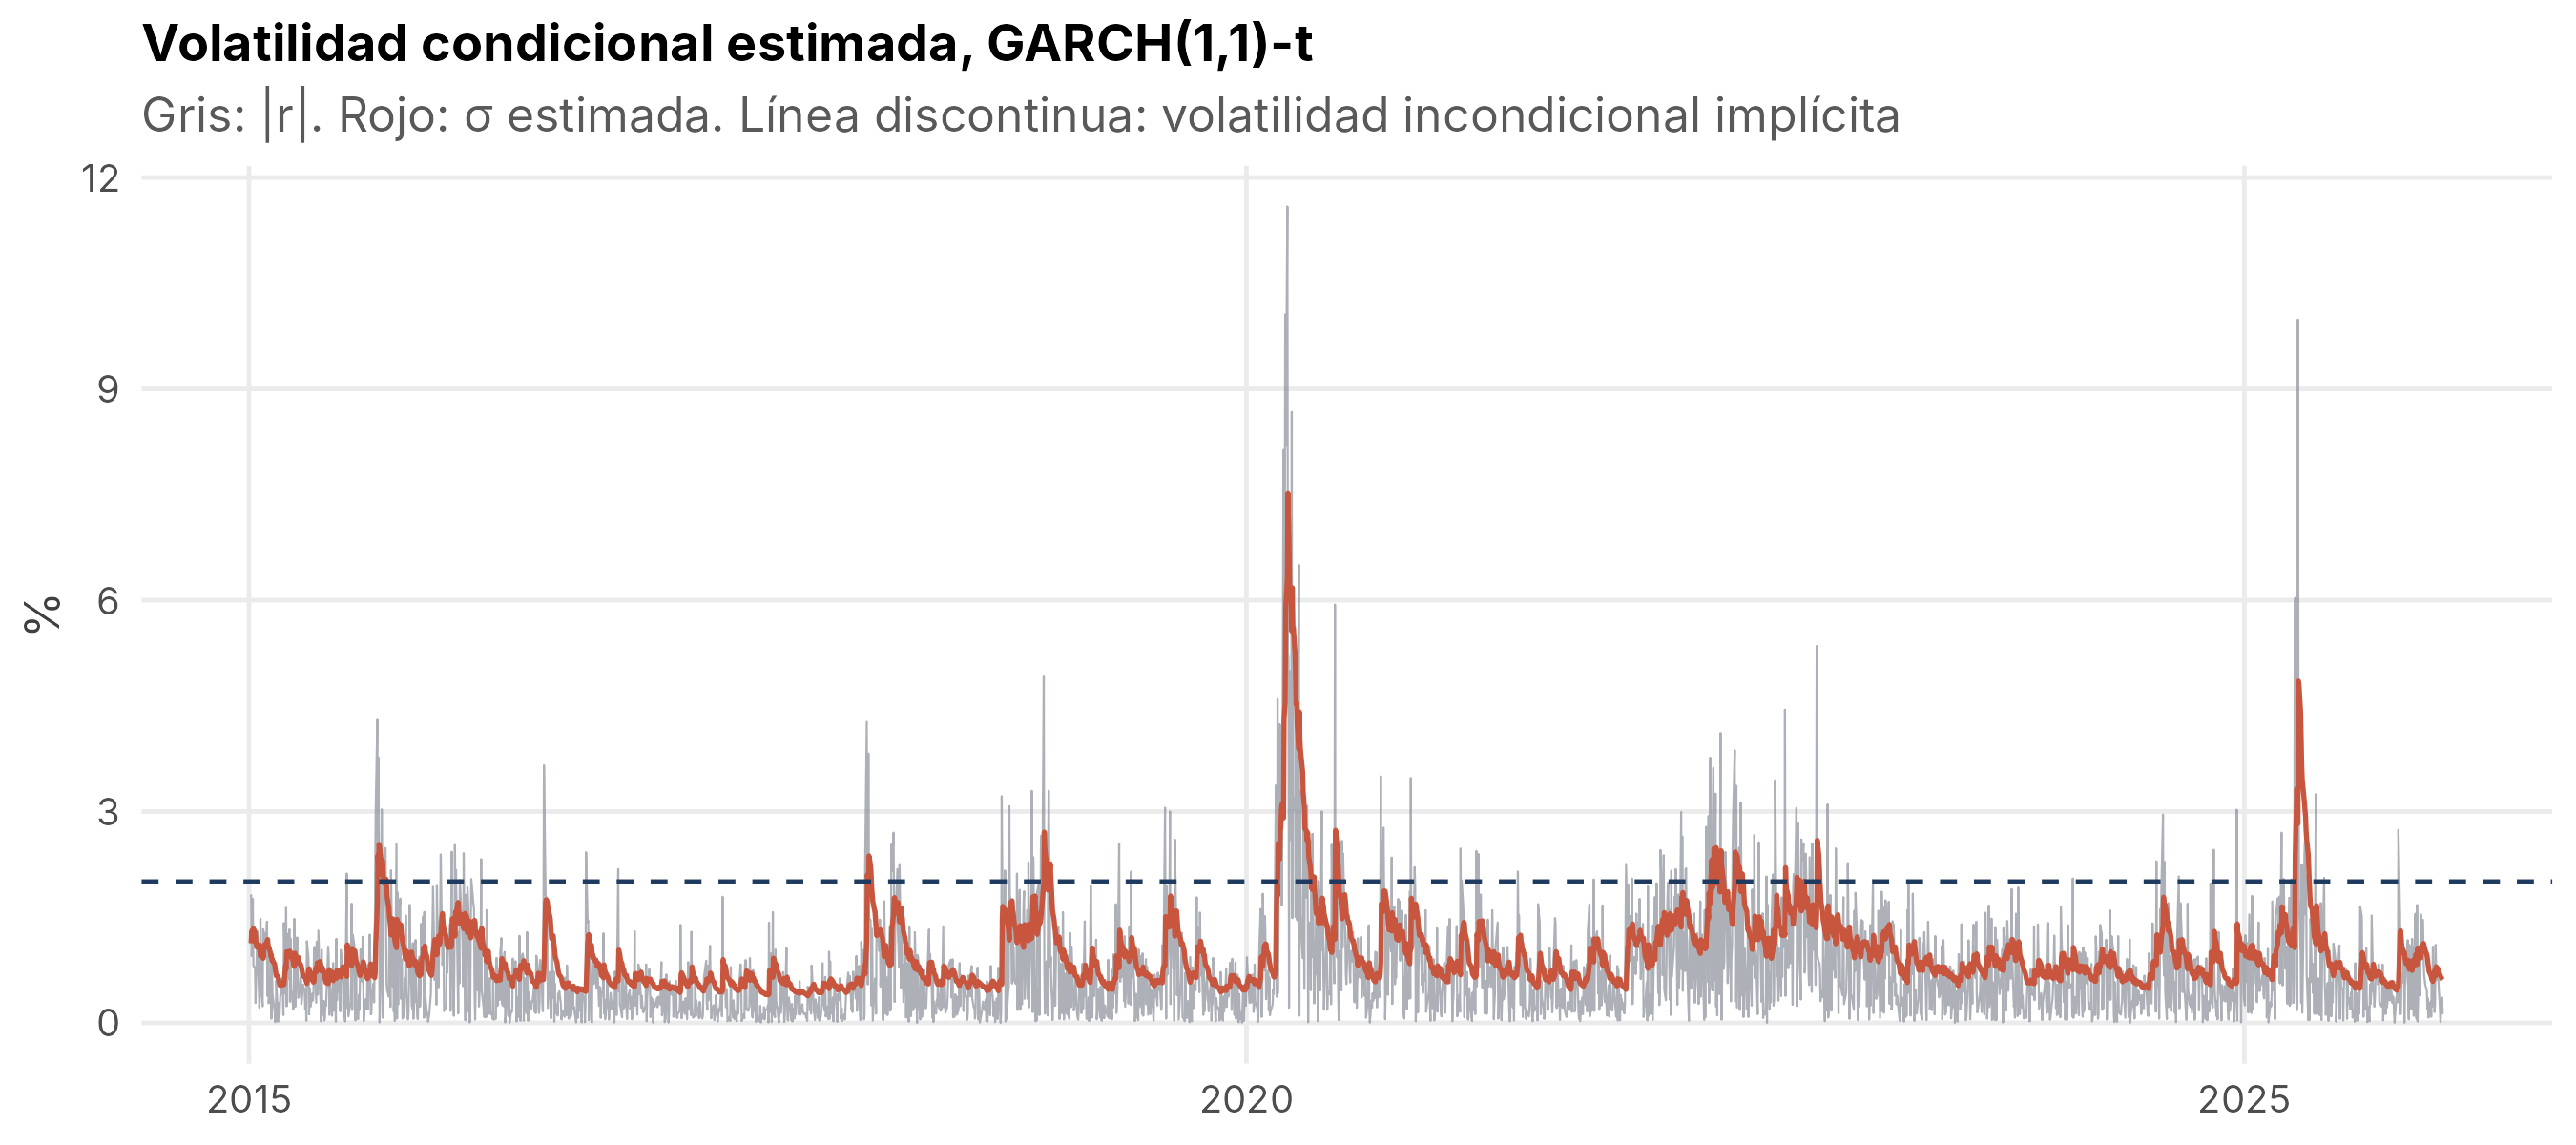
\includegraphics[width=0.88\linewidth]{f4_volatilidad_condicional.png}
\caption{Valor absoluto de los rendimientos y volatilidad condicional estimada $\hat\sigma_t$.}
\label{fig:vol}
\end{figure}

\begin{table}[H]
\centering\small
\caption{Pruebas sobre los residuales estandarizados del GARCH(1,1)-$t$.}
\label{tab:diag}
\begin{tabular}{lrr}
\toprule
Prueba sobre $\hat z_t$ & Estadístico & $p$-valor \\
\midrule
Ljung-Box $Q(10)$, $\hat z_t$ & 6{,}82 & 0{,}742 \\
Ljung-Box $Q(10)$, $\hat z_t^2$ & 12{,}54 & 0{,}128 \\
ARCH-LM(12) & 13{,}98 & 0{,}302 \\
Sesgo de signo (Engle-Ng), conjunta & 19{,}66 & $<0{,}001$ \\
\bottomrule
\end{tabular}

\end{table}

\begin{figure}[H]
\centering
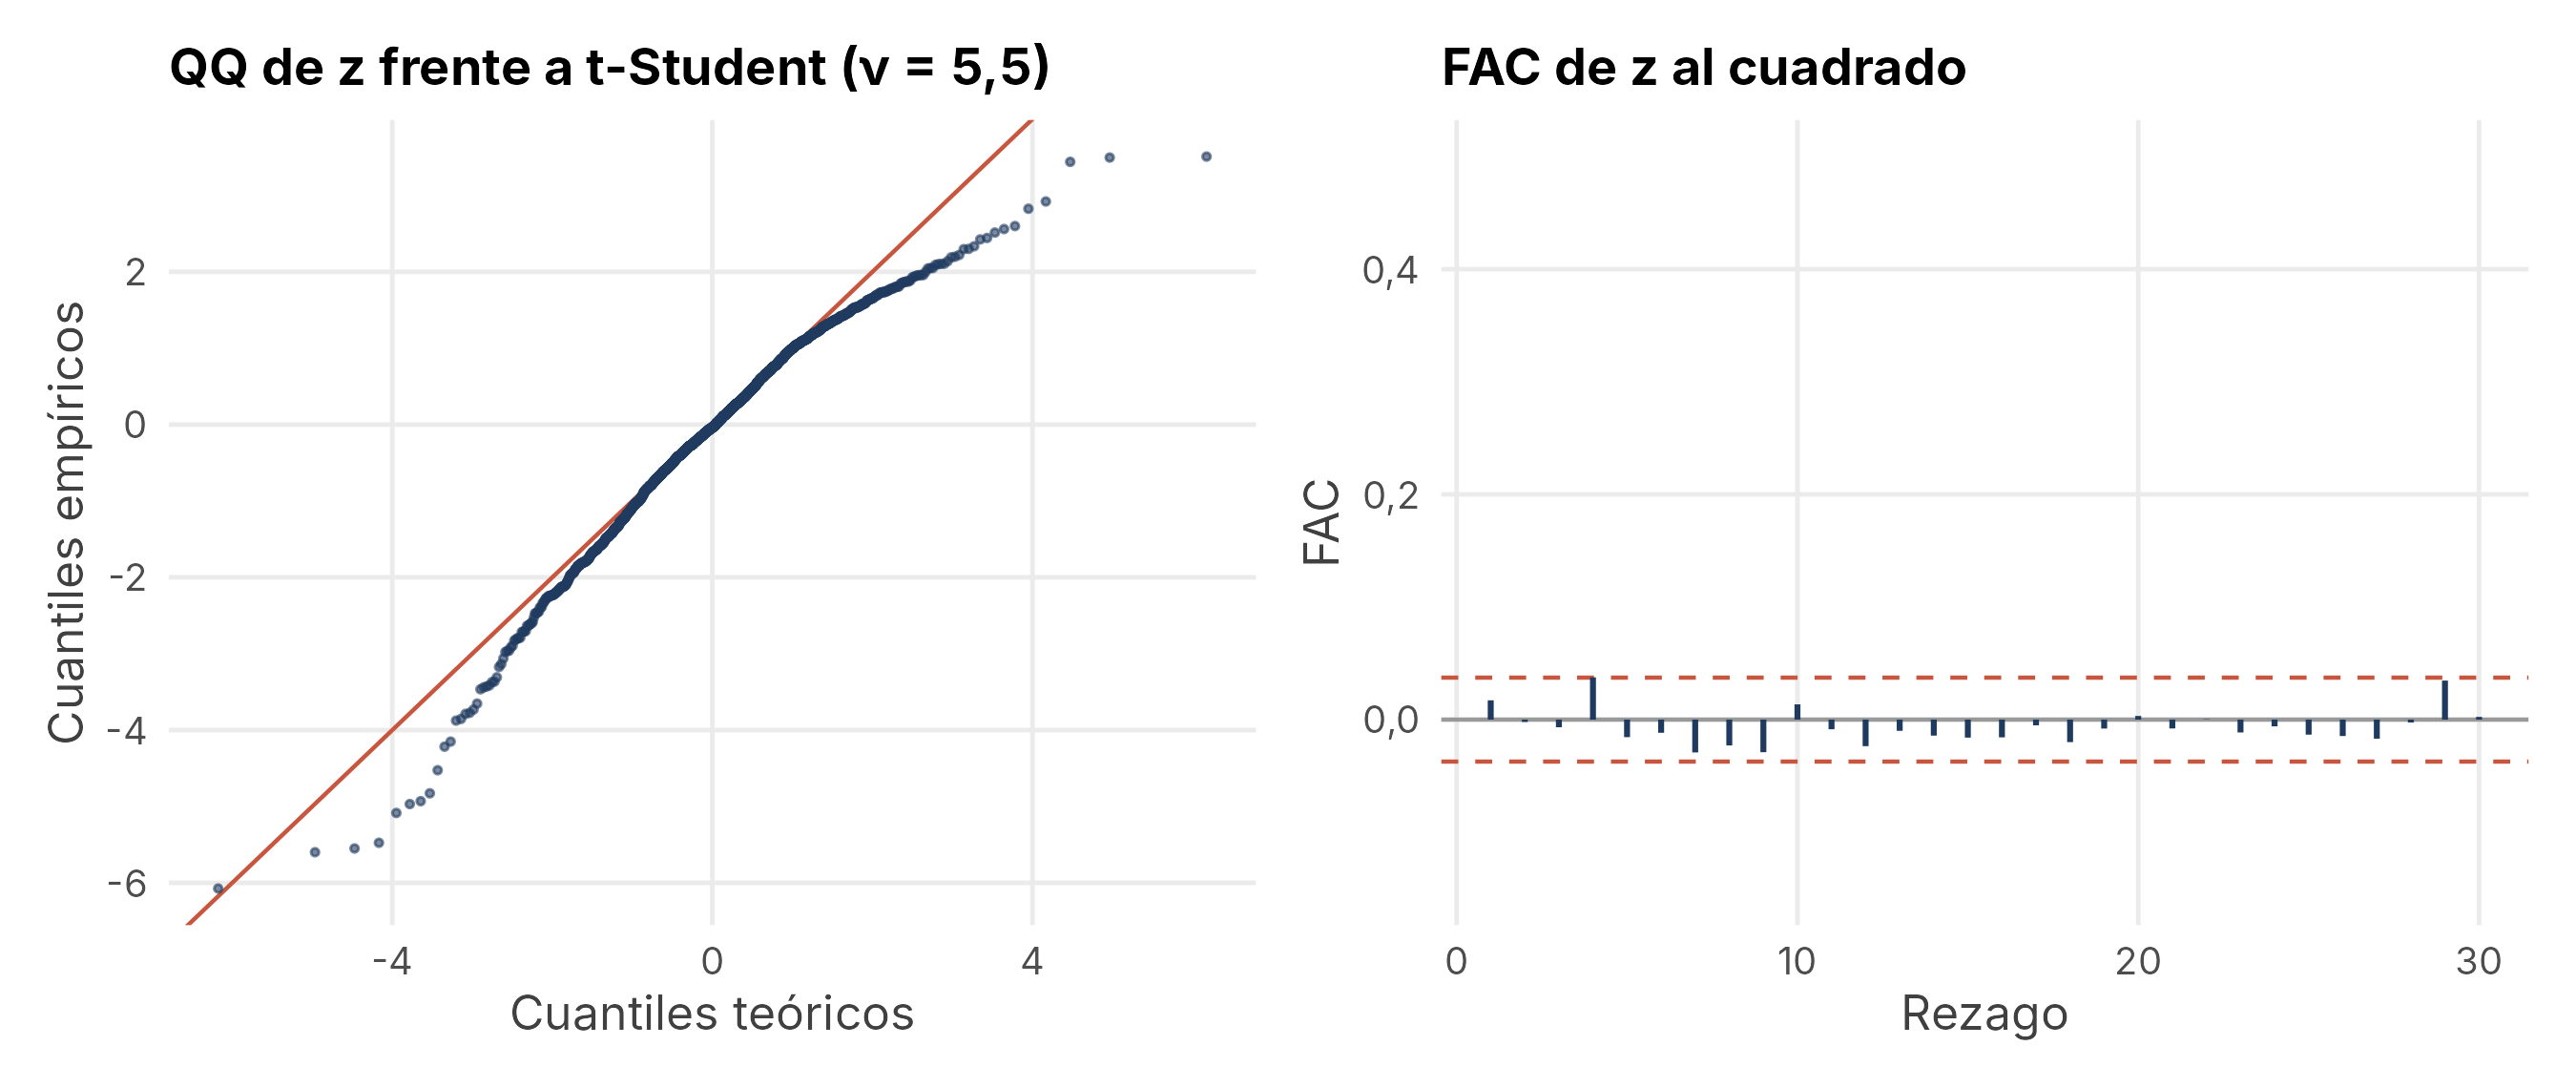
\includegraphics[width=0.88\linewidth]{f5_diagnostico.png}
\caption{Gráfico QQ de $\hat z_t$ frente a la $t$ estimada y FAC de $\hat z_t^2$.}
\label{fig:diag}
\end{figure}

\subsection{Pronóstico de la volatilidad}
Al cierre de 2025 el mercado estaba en calma: $\hat\sigma_{t+1}=\gSigmaUno$\,\% diario
(\gSigmaUnoAnual\,\% anualizado). Según~\eqref{eq:pronostico}, la volatilidad esperada
aumenta gradualmente hacia su nivel de largo plazo (figura~\ref{fig:pron}). A \gH{} días el
modelo libre pronostica \gSigmaH\,\% diario y el de \emph{variance targeting} \gSigmaHvt\,\%:
a corto plazo ambos coinciden, pero a largo plazo el pronóstico depende críticamente del
nivel incondicional, que es precisamente el parámetro peor identificado.

\begin{figure}[H]
\centering
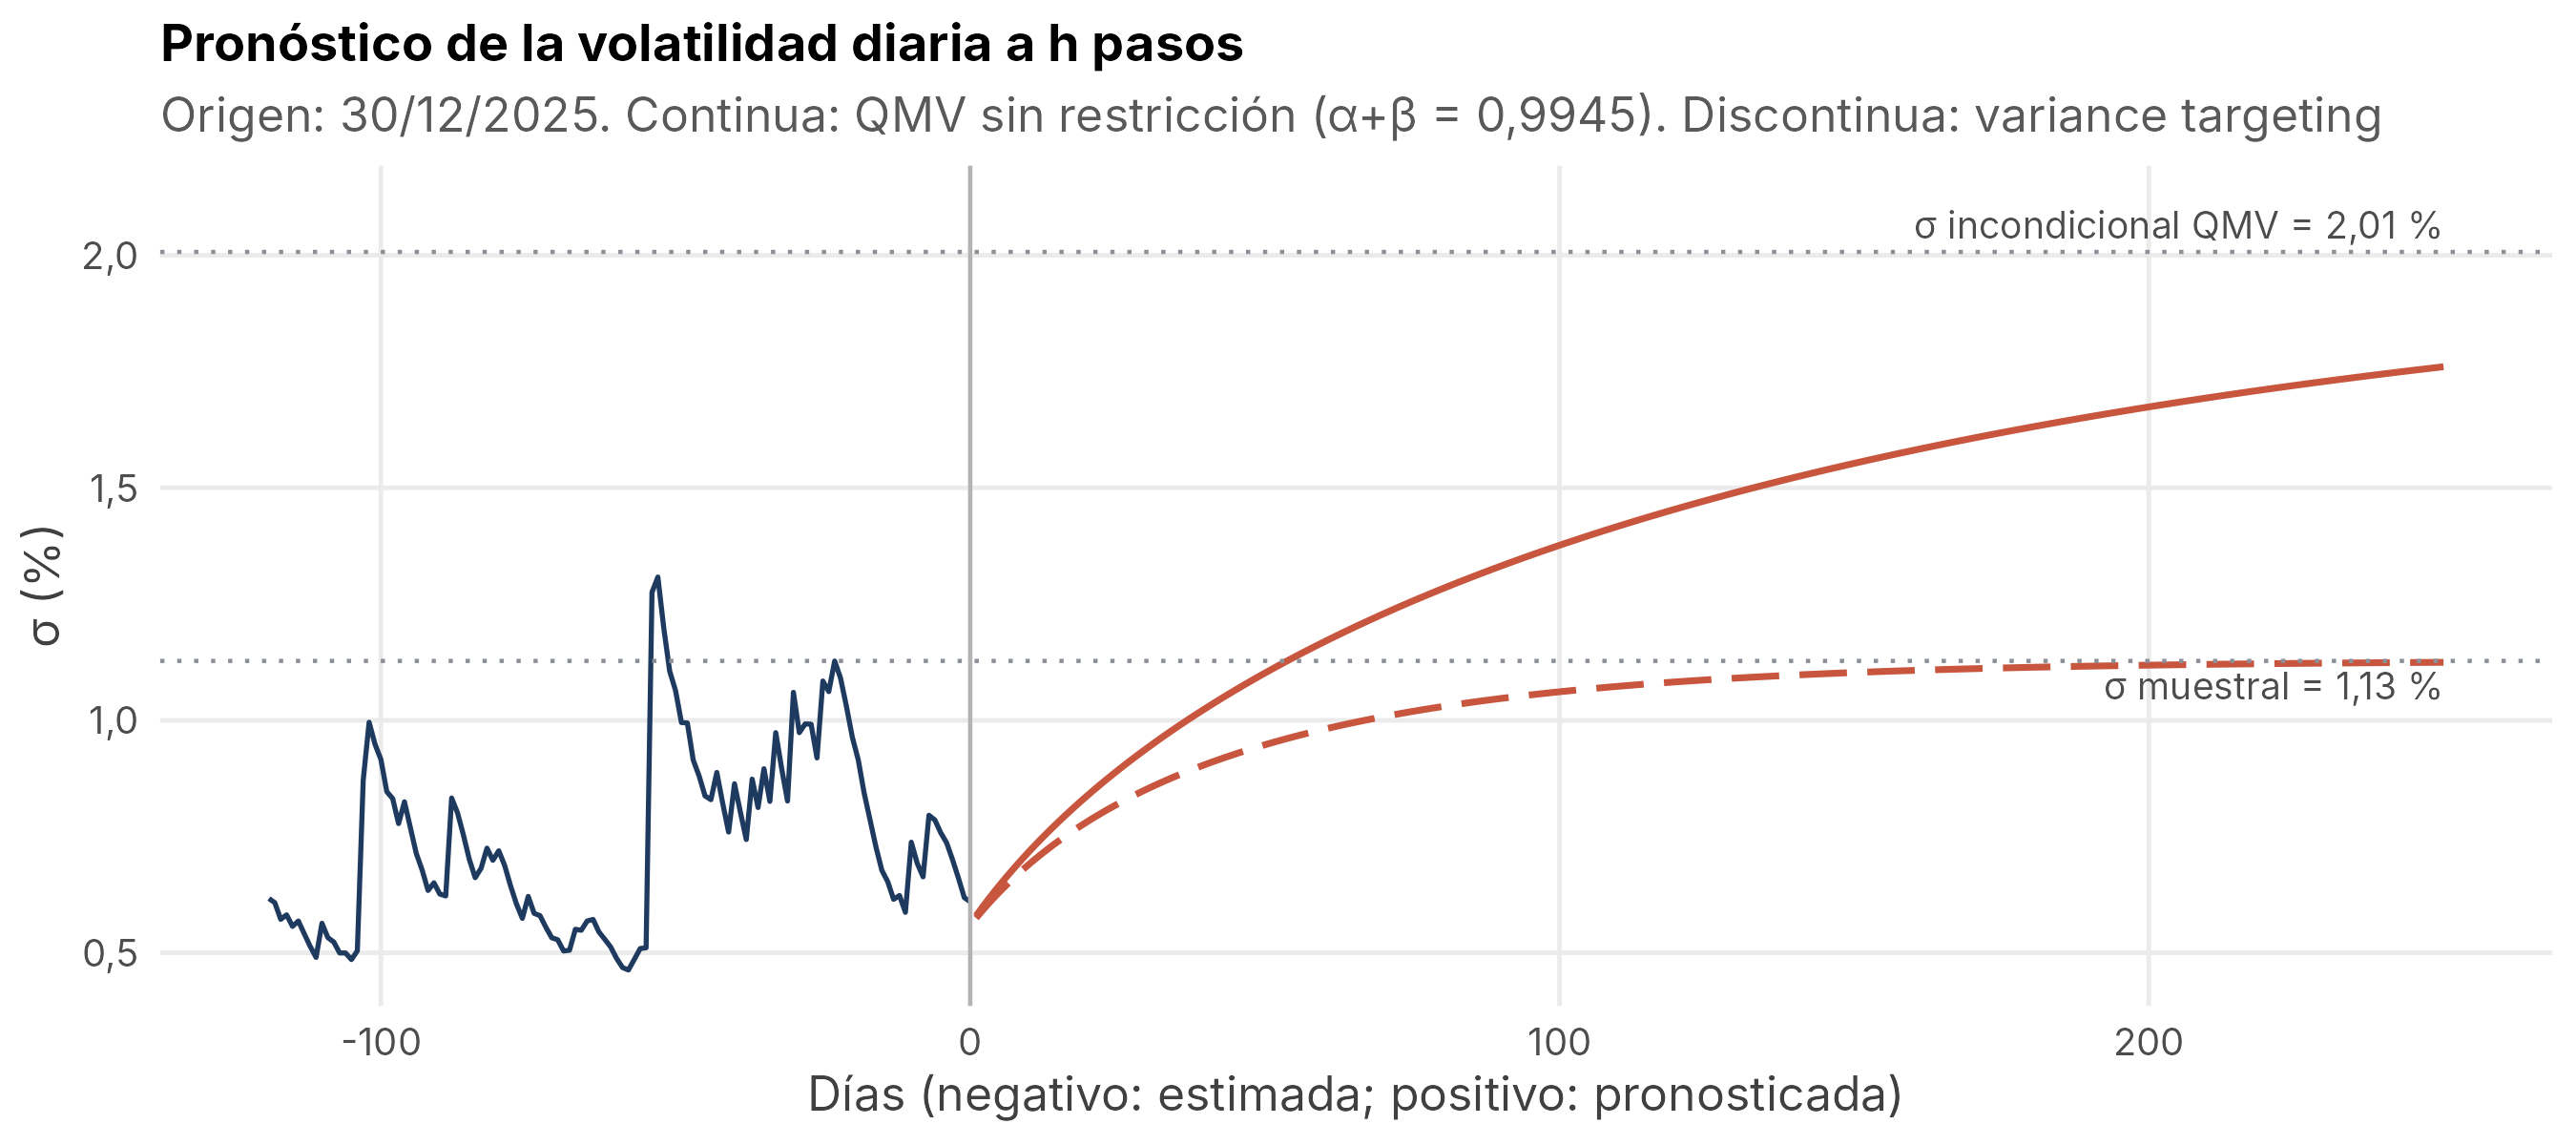
\includegraphics[width=0.88\linewidth]{f6_pronostico.png}
\caption{Volatilidad estimada en los últimos 120 días y pronosticada a 1--\gH{} días.}
\label{fig:pron}
\end{figure}

\subsection{Una posibilidad de uso: el Valor en Riesgo}
Con $\hat\sigma_{t+1}$ se obtiene cada día la pérdida que no debería superarse con
probabilidad $1-a$. La figura~\ref{fig:var} muestra cómo el VaR se ensancha
automáticamente en los periodos turbulentos, algo que un VaR con varianza constante no hace.
Según la tabla~\ref{tab:var}, al 1\,\% se observan \gExcUno{} excedencias frente a \gEspUno{}
esperadas y ninguna prueba rechaza. Al 5\,\% hay \gExcCinco{} frente a \gEspCinco: la prueba
de Kupiec rechaza al 5\,\% ($p=\gKupCincop$), aunque la de independencia no lo hace al mismo
nivel. Las excedencias no se agrupan en un episodio, sino que se reparten a lo largo de los dos
años, lo que apunta a un cuantil moderado mal calibrado más que a una reacción lenta del modelo.
Dos causas plausibles: la $t$ estandarizada con $\hat\nu=\gNu$ concentra masa en el centro y en
los extremos, por lo que su cuantil del 5\,\% es menos negativo que el de la normal
($-1{,}58$ frente a $-1{,}64$), y la distribución supuesta es simétrica, mientras que los
rendimientos tienen asimetría negativa.

\begin{figure}[H]
\centering
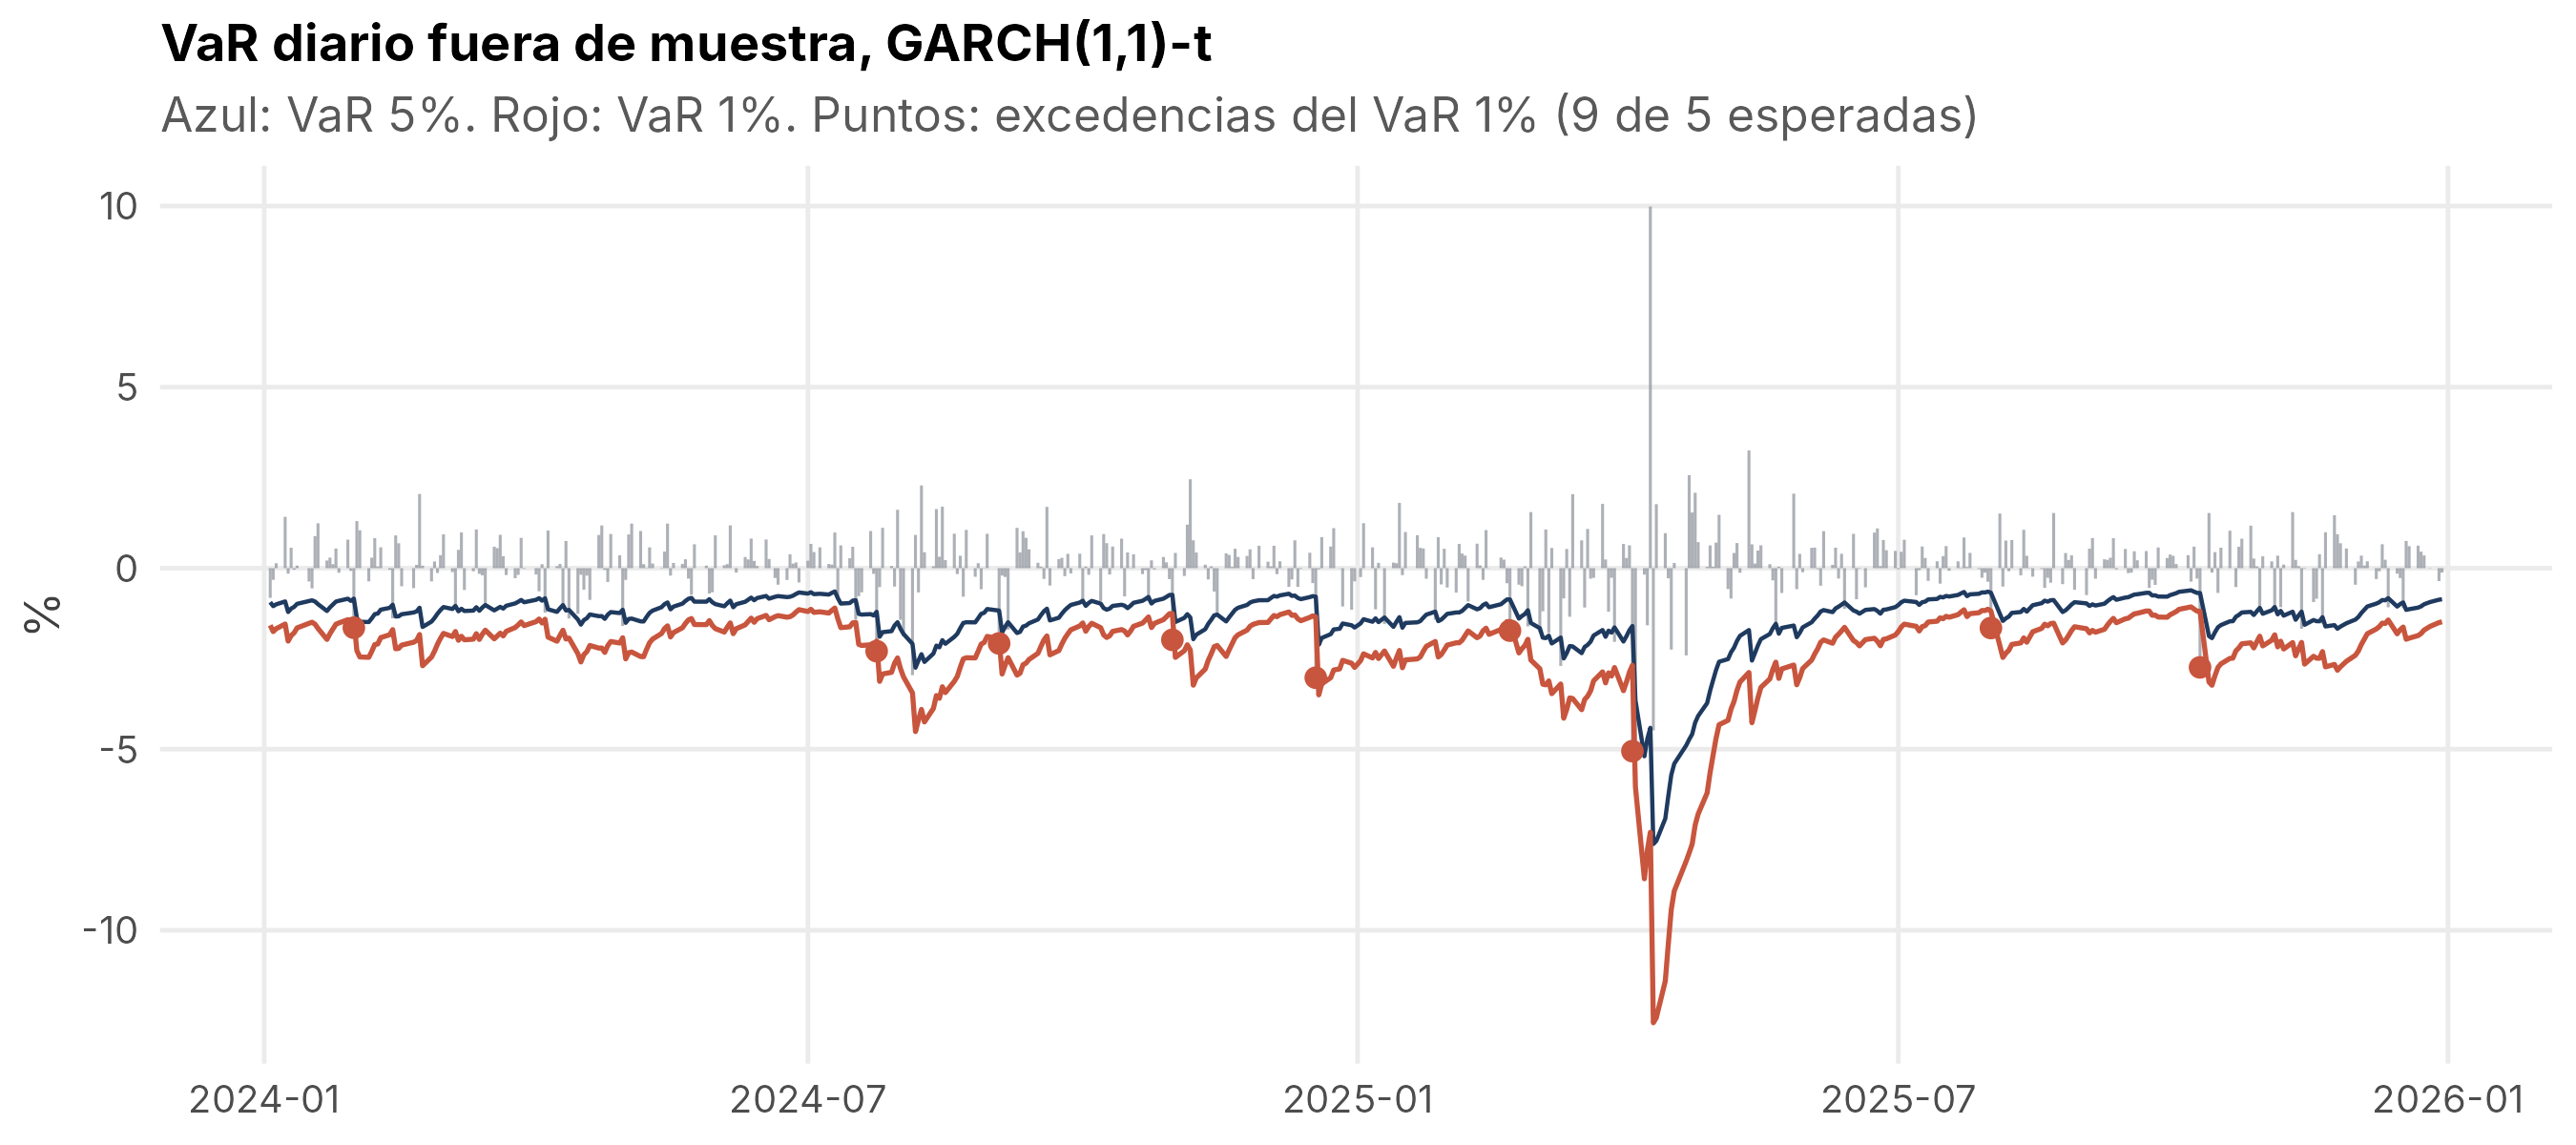
\includegraphics[width=0.88\linewidth]{f7_var_backtesting.png}
\caption{Rendimientos y VaR diario a un paso fuera de muestra (2024--2025).}
\label{fig:var}
\end{figure}

\begin{table}[H]
\centering\small
\caption{Evaluación del VaR fuera de muestra (\gOosN{} días).}
\label{tab:var}
\begin{tabular}{lrrrrrr}
\toprule
 & \multicolumn{2}{c}{Excedencias} & \multicolumn{2}{c}{Kupiec} & \multicolumn{2}{c}{Christoffersen} \\
\cmidrule(lr){2-3}\cmidrule(lr){4-5}\cmidrule(lr){6-7}
Nivel & Esperadas & Observadas & LR & $p$-valor & LR & $p$-valor \\
\midrule
1\% & 5 & 9 & 2{,}61 & 0{,}106 & 2{,}94 & 0{,}230 \\
5\% & 25 & 36 & 4{,}51 & 0{,}034 & 4{,}68 & 0{,}096 \\
\bottomrule
\end{tabular}

\end{table}

%%%%%%%%%%%%%%%%%%%%%%%%%%%%%%%%%%%%%%
\section{Conclusiones}

\textbf{Teoría frente a resultados.}
\begin{itemize}
  \item Los rendimientos del S\&P 500 cumplen los hechos estilizados que motivan el modelo:
  incorrelación débil, fuerte dependencia en los cuadrados, agrupamiento de volatilidad y colas
  pesadas.
  \item Como anticipa la representación ARCH$(\infty)$, tres parámetros de varianza bastan: el
  GARCH(1,1) no mejora al aumentar los órdenes y elimina la heterocedasticidad condicional de
  los residuales.
  \item Los parámetros estimados satisfacen la condición de estacionariedad estricta y, en la
  estimación puntual, la de segundo orden, pero no la de cuarto momento. La persistencia
  (\gPersist) no se distingue estadísticamente del caso IGARCH, en el que la varianza
  incondicional deja de existir.
  \item La cercanía a la raíz unitaria tiene una consecuencia práctica: el nivel de largo plazo,
  y por tanto el pronóstico a horizontes largos, es poco confiable, como muestra la
  comparación con \emph{variance targeting}.
\end{itemize}

\textbf{Ventajas.} Parsimonia; parámetros con interpretación directa (reacción, memoria,
persistencia); pronósticos en forma cerrada; estimación estándar con teoría asintótica
conocida, y un vínculo inmediato con medidas de riesgo como el VaR.

\textbf{Desventajas.} Respuesta simétrica a choques positivos y negativos (rechazada por la
prueba de sesgo de signo); restricciones de positividad sobre los parámetros; dificultad para
identificar el nivel de largo plazo cuando la persistencia es alta, que puede confundirse con
cambios estructurales; innovaciones simétricas que calibran mal los cuantiles moderados de
pérdida (VaR al 5\,\%), y formulación univariada.

\textbf{Posibilidad de uso.} Cualquier decisión que dependa de cuánto puede moverse un
activo mañana puede apoyarse en un GARCH: fijar límites de pérdida o márgenes con el VaR,
ajustar el tamaño de una posición para mantener constante su riesgo, o alimentar la
volatilidad de un modelo de valoración de opciones. Las limitaciones encontradas indican
cómo mejorarlo: modelos asimétricos (EGARCH, GJR) para el efecto apalancamiento y
especificaciones que permitan cambios en el nivel de largo plazo.

%%%%%%%%%%%%%%%%%%%%%%%%%%%%%%%%%%%%%%
\renewcommand{\refname}{Referencias bibliográficas}
\begin{thebibliography}{99}
\setlength{\itemsep}{0.1em}\small

\bibitem[Bollerslev(1986)]{bollerslev1986}
Bollerslev, T. (1986). Generalized autoregressive conditional heteroskedasticity.
\emph{Journal of Econometrics}, 31(3), 307--327.

\bibitem[Bollerslev y Wooldridge(1992)]{bollerslev1992}
Bollerslev, T. y Wooldridge, J. M. (1992). Quasi-maximum likelihood estimation and inference
in dynamic models with time-varying covariances. \emph{Econometric Reviews}, 11(2), 143--172.

\bibitem[Bougerol y Picard(1992)]{bougerol1992}
Bougerol, P. y Picard, N. (1992). Stationarity of GARCH processes and of some nonnegative
time series. \emph{Journal of Econometrics}, 52(1--2), 115--127.

\bibitem[Christoffersen(1998)]{christoffersen1998}
Christoffersen, P. F. (1998). Evaluating interval forecasts. \emph{International Economic
Review}, 39(4), 841--862.

\bibitem[Engle(1982)]{engle1982}
Engle, R. F. (1982). Autoregressive conditional heteroscedasticity with estimates of the
variance of United Kingdom inflation. \emph{Econometrica}, 50(4), 987--1007.

\bibitem[Engle y Mezrich(1996)]{engle1996}
Engle, R. F. y Mezrich, J. (1996). GARCH for groups. \emph{Risk}, 9(8), 36--40.

\bibitem[Engle y Ng(1993)]{engle1993}
Engle, R. F. y Ng, V. K. (1993). Measuring and testing the impact of news on volatility.
\emph{The Journal of Finance}, 48(5), 1749--1778.

\bibitem[Francq y Zakoïan(2004)]{francq2004}
Francq, C. y Zakoïan, J.-M. (2004). Maximum likelihood estimation of pure GARCH and
ARMA-GARCH processes. \emph{Bernoulli}, 10(4), 605--637.

\bibitem[Francq y Zakoïan(2010)]{francq2010}
Francq, C. y Zakoïan, J.-M. (2010). \emph{GARCH Models: Structure, Statistical Inference and
Financial Applications}. Chichester: John Wiley \& Sons.

\bibitem[Ghalanos(2026)]{ghalanos}
Ghalanos, A. (2026). \emph{rugarch: Univariate GARCH Models}. Paquete de R, versión \gRugarch.
\url{https://CRAN.R-project.org/package=rugarch}

\bibitem[Jarque y Bera(1980)]{jarque1980}
Jarque, C. M. y Bera, A. K. (1980). Efficient tests for normality, homoscedasticity and serial
independence of regression residuals. \emph{Economics Letters}, 6(3), 255--259.

\bibitem[Kupiec(1995)]{kupiec1995}
Kupiec, P. H. (1995). Techniques for verifying the accuracy of risk measurement models.
\emph{The Journal of Derivatives}, 3(2), 73--84.

\bibitem[Lamoureux y Lastrapes(1990)]{lamoureux1990}
Lamoureux, C. G. y Lastrapes, W. D. (1990). Persistence in variance, structural change, and
the GARCH model. \emph{Journal of Business \& Economic Statistics}, 8(2), 225--234.

\bibitem[Ljung y Box(1978)]{ljung1978}
Ljung, G. M. y Box, G. E. P. (1978). On a measure of lack of fit in time series models.
\emph{Biometrika}, 65(2), 297--303.

\bibitem[Nelson(1990)]{nelson1990}
Nelson, D. B. (1990). Stationarity and persistence in the GARCH(1,1) model.
\emph{Econometric Theory}, 6(3), 318--334.

\bibitem[R Core Team(2024)]{rcore}
R Core Team (2024). \emph{R: A Language and Environment for Statistical Computing}. Viena:
R Foundation for Statistical Computing. \url{https://www.R-project.org}

\bibitem[Rossi(2013)]{rossi2013}
Rossi, E. (2013). \emph{GARCH Models}. Notas del curso Financial Econometrics, Universidad de
Pavía.

\bibitem[Twelve Data(2026)]{twelvedata}
Twelve Data (2026). \emph{Time Series API}: precios diarios del SPDR S\&P 500 ETF (SPY).
\url{https://twelvedata.com}. Consultado en noviembre de 2026.

\end{thebibliography}

\end{document}
